\lstset{style=Python,basicstyle=\ttfamily\footnotesize}

\begin{frame}
    \centering
    \begin{figure}[H]
        \includegraphics[keepaspectratio, width=0.7\paperwidth, height=\paperheight]{\thelogo}
    \end{figure}
    Informatik: Programmieren\\
    \emoji{cook} Kapitel 04: \textbf{Neue Funktionen definieren}
\end{frame}

% command to make sure colorboxes don't create whitespace between code lines
\fboxsep=.6pt


\begin{frame}[fragile]{Wiederholung letztes Mal}
\begin{lstlisting}[escapechar=!]
import turtle as t

for _ in range(6):!\tikzmark{repeatStart}!
    t.fd(100)!\tikzmark{code2}!  !\tikzmark{bodyStart}!                                !\tikzmark{comment2}!
    t.rt(360/6)!\tikzmark{code3}! !\tikzmark{bodyEnd}!                   !\tikzmark{comment3}!
\end{lstlisting}
\begin{itemize}[<+->]
\item Wie nennt man die Ausdrücke auf den Zeilen 4 und 5? % Antwort: Befehl
\item Wie nennt man Zeilen 3 bis 5? % Antwort: Schleife
\item Wie nennt man Zeilen 4-5? % Antwort: Körper der Schleife
\end{itemize}

\begin{tikzpicture}[overlay, remember picture,
    every node/.style={draw=red!50,fill=red!50!white,text=black,rounded corners}]
\only<2->{
    \drawArrow{code2}{comment2}{\footnotesize\emoji{cook} Befehl / Funktion}{RoyalBlue!50!white};
    \drawArrow{code3}{comment3}{\footnotesize\emoji{cook} Befehl / Funktion}{RoyalBlue!50!white};}
    \only<3->{\drawBrace{1em}{repeatStart}{bodyEnd}{\footnotesize Schleife}{.3}{}{};}
    \only<4->{\drawBrace{.0em}{bodyStart}{bodyEnd}{\textit{\footnotesize Körper} der Schleife}{.7}{}{};}
\end{tikzpicture}
\only<5->{\begin{itemize}
\item Mit \textbf{Funktionen} können wir den Computer eine abstrakte Tätigkeit ausführen lassen
\item \textbf{Parameter} dienen dazu, die Funktionen \textit{parametrisieren} (Analogie: Kochrezept für 2 oder 4 Personen)
\item \textbf{Schleifen} erlauben es, repetitive Tätigkeiten kompakt zu beschreiben
\item Unterschiedliche \textbf{Datentypen} für unterschiedliche Zwecke
\end{itemize}}
\end{frame}

\begin{frame}[fragile]{Neue Funktion definieren}
\begin{lstlisting}[escapechar=!]
import turtle as t

# zeichne ein Quadrat
for _ in range(4):      !\tikzmark{befehlStart}!
    t.fd(100)  # Funktion  
    t.rt(90)   # Funktion !\tikzmark{befehlEnde}!
    
t.done()
\end{lstlisting}
\begin{tikzpicture}[overlay, remember picture,
    every edge/.append style = { ->, thick, >=stealth, red!70},
    every node/.style={draw=red!50,fill=red!50!white,text=black,rounded corners}]
    \only<2->{\drawBrace{0em}{befehlStart}{befehlEnde}{Neue Funktion für alles?}{.5}{}{};}
\end{tikzpicture}
\end{frame}

\begin{frame}[fragile]{Neue Funktionen definieren}
\begin{lstlisting}[escapechar=!]
import turtle as t

def quadr!\tikzmark{to}!at():         !\tikzmark{befehlStart}!
    for _ in range(4):
        t.fd(100)
        t.rt(90)       !\tikzmark{befehlEnde}!

quadrat()!\tikzmark{from1}!
t.rt(45)
quadrat()!\tikzmark{from2}!

t.done()
\end{lstlisting}
\begin{tikzpicture}[overlay, remember picture,
    every edge/.append style = { ->, thick, >=stealth, red!70},
    every node/.style={draw=red!50,fill=red!50!white,text=black,rounded corners}]
	\drawBrace{0em}{befehlStart}{befehlEnde}{Funktion wird definiert \emoji{page-facing-up}}{.5}{}{};
\end{tikzpicture}
\begin{itemize}
\item Definition = \lstinline|def| = Funktion
\item Ähnlich einem Kochrezept \emoji{page-facing-up}
\begin{itemize}
\item Beschreibung der auzuführenden Schritte
\item Wird erst ausgeführt, sobald aufgerufen! \emoji{cook}
\end{itemize}
\only<2->{
\begin{tikzpicture}[overlay,remember picture]
\draw[red,-stealth] (from1.north) to[bend right] node[below=.6cm, xshift=.8cm, fill=CornflowerBlue,rounded corners] {\emoji{cook} Aufruf} (to);
\draw[red,-stealth] (from2.north) to[bend right] node[below=.9cm, xshift=.7cm, fill=CornflowerBlue, rounded corners] {\emoji{cook} Aufruf} (to);
\end{tikzpicture}}
\end{itemize}
\end{frame}

\begin{frame}[fragile]{Viereck-Blume}
\begin{center}
\begin{minipage}{.4\textwidth}
\begin{lstlisting}[escapechar=!]
import turtle as t

for _ in range(10):   !\tikzmark{repOuterStart}!
    for _ in range(4):!\tikzmark{repInnerStart}!
        t.fd(100)
        t.rt(360 / 4) !\tikzmark{repInnerEnd}!
    t.rt(360 / 10)    !\tikzmark{repOuterEnd}!
    
t.done()
\end{lstlisting}
\begin{figure}[H]
\centering
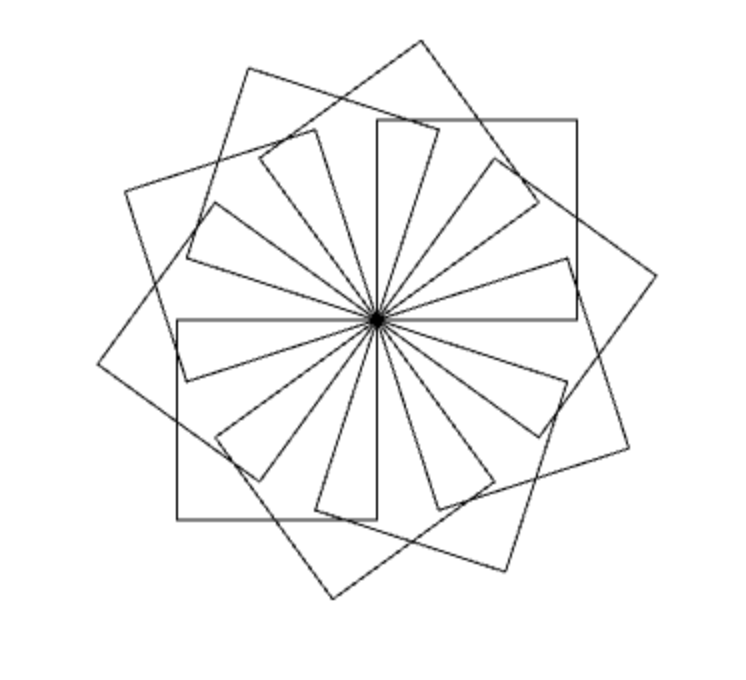
\includegraphics[width=0.6\textwidth]{Grundlagen_Info/00_Programmieren/Figures/viereck_blume}
\end{figure}
\end{minipage}\hfill\begin{minipage}{.4\textwidth}
\begin{lstlisting}[escapechar=!]
import turtle as t

!\tikzmark{repInnerStartTo}!def viereck():
    for _ in range(4):
        t.fd(100)
!\tikzmark{repInnerEndTo}!        t.rt(360 / 4)

!\tikzmark{repOuterStartTo}!def viereck_blume():
    for _ in range(10):
        viereck()
!\tikzmark{repOuterEndTo}!        t.rt(360/10)

viereck_blume()

t.done()
\end{lstlisting}
\end{minipage}
\end{center}
\begin{tikzpicture}[overlay, remember picture,
    every edge/.append style = { ->, thick, >=stealth, red!70},
    every node/.style={draw=red!50,fill=red!50!white,text=black,rounded corners}]
	\drawBrace{0em}{repInnerStart}{repInnerEnd}{}{.5}{};
		\drawBrace{-.5em}{repInnerStartTo}{repInnerEndTo}{}{.5}{mirror};
		% arrow pointing from one code to other
		\draw[->, style={thick, >=stealth, red!70}] (repInnerStartrepInnerEnd-coord-arrow) to (repInnerStartTorepInnerEndTo-coord-arrow);
		\drawBrace{1em}{repOuterStart}{repOuterEnd}{}{.75}{};
			\drawBrace{-.5em}{repOuterStartTo}{repOuterEndTo}{}{.25}{mirror};
			% arrow pointing from one code to other
			\draw[->, style={thick, >=stealth, red!70}] (repOuterStartrepOuterEnd-coord-arrow) to (repOuterStartTorepOuterEndTo-coord-arrow);
\end{tikzpicture}
\end{frame}

\begin{frame}[fragile]{Neue Funktionen definieren}
\begin{columns}
\begin{column}{.48\textwidth}
\begin{lstlisting}[escapechar=!]
import turtle as t

def !\only<1-2>{viereck()}\only<3->{\colorbox{CarnationPink}{viereck()}}!: !\tikzmark{to2ex}!
    for _ in range(4):
        t.fd(100)
        t.rt(360/4)

def !\only<1>{viereck\_blume()}\only<2->{\colorbox{CornflowerBlue}{viereck\_blume()}}!:!\tikzmark{to1ex}! 
    for _ in range(10):
        !\only<1-2>{viereck()}\only<3->{\colorbox{CarnationPink}{viereck()}}! !\tikzmark{from2ex}!
        t.rt(360/10)

!\only<1>{viereck\_blume()}\only<2->{\colorbox{CornflowerBlue}{viereck\_blume()}}! !\tikzmark{from1ex}!
\end{lstlisting}
\begin{tikzpicture}[overlay,remember picture]
\only<2->{\draw[red,-stealth] (from1ex.north) to[bend right] node[fill=CornflowerBlue,rounded corners] {\emoji{cook} Aufruf} (to1ex);}
\only<3->{\draw[red,-stealth] (from2ex.north) to[bend right] node[fill=CornflowerBlue,rounded corners] {\emoji{cook} Aufruf} (to2ex);}
\end{tikzpicture}
\end{column}
\begin{column}{.5\textwidth}
\begin{figure}[H]
\centering
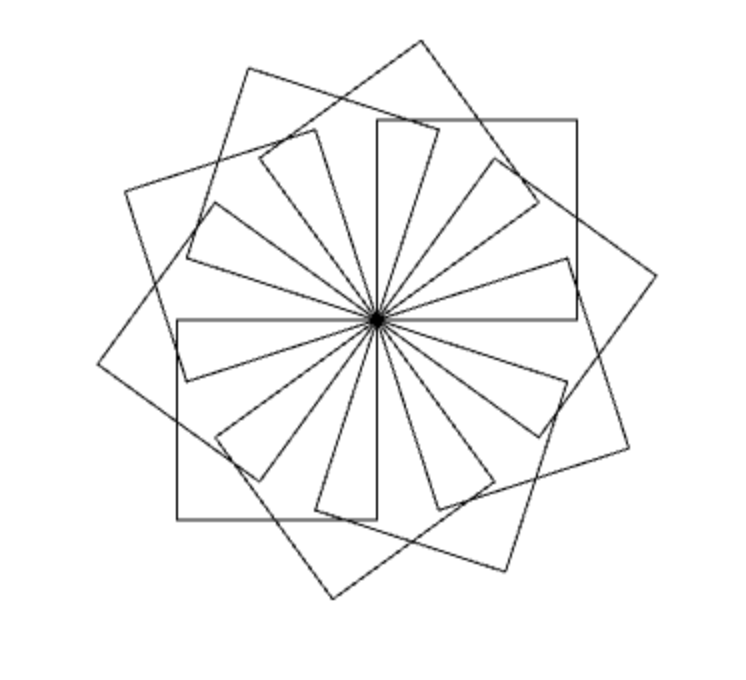
\includegraphics[width=0.6\columnwidth]{Grundlagen_Info/00_Programmieren/Figures/viereck_blume}
\end{figure}
\begin{itemize}
\item \textbf{Modularität}: Zerlegung des Programms in kleinere Stücke
\item \textbf{Übersichtlicher}!
\end{itemize}
\end{column}
\end{columns}
\end{frame}

\begin{frame}[fragile]{Funktionen \& Schleifen}
\begin{columns}
\begin{column}[t]{.5\textwidth}
\begin{lstlisting}[escapechar=!,basicstyle=\ttfamily\footnotesize]
import turtle as t

for _ in range(4):      !\tikzmark{repOuterStart}!
    for _ in range(9):  !\tikzmark{repInnerStart}!
        t.fd(4)
        t.lt(10)        !\tikzmark{repInnerEnd}!
    t.fd(100)           !\tikzmark{repOuterEnd}!
    
t.done()
\end{lstlisting}
\begin{center}

\includegraphics[width=0.3\linewidth]{Grundlagen_Info/00_Programmieren/Figures/round-circle}
\end{center}
\only<4->{
\footnotesize
\textbf{Übersichtlichkeit}
\begin{itemize}
\item Innere Schleifen $\rightarrow$ Funktionen
\item Sprechende Definitions-Namen
\end{itemize}
}
\end{column}
\begin{column}[t]{.5\textwidth}
\begin{lstlisting}[escapechar=!,basicstyle=\ttfamily\footnotesize]
import turtle as t

!\tikzmark{repInnerStartTo}!def viertelkreis():
    for _ in range(9):
        t.fd(4)
!\tikzmark{repInnerEndTo}!        t.lt(10)

!\tikzmark{repOuterStartTo}!def abgerundetes_quadrat():
	for _ in range(4):
        viertelkreis()
!\tikzmark{repOuterEndTo}!        t.fd(100)

abgerundetes_quadrat()

t.done()
\end{lstlisting}
\end{column}
\end{columns}
\begin{tikzpicture}[overlay, remember picture,
    every edge/.append style = { ->, thick, >=stealth, red!70},
    every node/.style={draw=red!50,fill=red!50!white,text=black,rounded corners}]
	\only<2->{
	\drawBrace{0em}{repInnerStart}{repInnerEnd}{}{.5}{};
		\drawBrace{-.5em}{repInnerStartTo}{repInnerEndTo}{}{.5}{mirror};
		% arrow pointing from one code to other
		\draw[->, style={thick, >=stealth, red!70}] (repInnerStartrepInnerEnd-coord-arrow) to (repInnerStartTorepInnerEndTo-coord-arrow);
		}
	\only<3->{
		\drawBrace{1em}{repOuterStart}{repOuterEnd}{}{.75}{};
			\drawBrace{-.5em}{repOuterStartTo}{repOuterEndTo}{}{.25}{mirror};
			% arrow pointing from one code to other
			\draw[->, style={thick, >=stealth, red!70}] (repOuterStartrepOuterEnd-coord-arrow) to (repOuterStartTorepOuterEndTo-coord-arrow);
			}
\end{tikzpicture}
\end{frame}

\begin{frame}[fragile]{Zusammenfassung}
Nutzen von \textbf{Funktionen}
\begin{itemize}[<+->]
\item Problem in \textbf{Teilprobleme} gliedern
\item \textbf{Übersichtlichkeit} erhöhen
\item \textbf{Sinnstiftender} Name für jede Definition!
\item Im ``Hauptprogramm'' Funktionen zusammensetzen
\end{itemize}
\end{frame}

\begin{frame}[fragile]{Auftrag: Skript, Kapitel 4}
\begin{itemize}
\item Skript immer zuerst durchlesen \emoji{wink}
\begin{quote}
\enquote{
\textit{A small step for students but a giant leap for the teacher...}
}
\end{quote}
\item Übungen in VSCodium und auf Moodle lösen
\item \aufgabebox{Aufgaben 4.1, 4.2}
\item \abgabebox{Moodle-Test \enquote{Kapitel 4 (Teil 1)}}
\end{itemize}


\end{frame}

